%https://tex.stackexchange.com/questions/164991/pgfplots-how-to-fill-bounded-area-under-a-curve-using-addplot-and-fill

%https://tex.stackexchange.com/questions/140312/tikz-shading-region-bounded-by-several-curves
%tikz para graficar areas

%http://latexcolor.com/

%https://www.tablesgenerator.com/
\PassOptionsToPackage{force}{filehook}

\documentclass{beamer}


\usepackage[utf8]{inputenc}
\usepackage{amsmath}
\usepackage{amssymb}% http://ctan.org/pkg/amssymb
\usepackage{amsfonts}
\usepackage{pifont}% http://ctan.org/pkg/pifont
%https://tex.stackexchange.com/questions/42619/x-mark-to-match-checkmark
\newcommand{\cmark}{\ding{51}}
\newcommand{\xmark}{\ding{55}}
%\usepackage{amsfonts}
\usepackage{graphicx} 
\usepackage{subcaption}
\usepackage{hyperref}
\usepackage{cancel}
\usepackage{wrapfig}
\usepackage{enumitem}
\usepackage{comment}
\hypersetup{
	colorlinks=true,
	linkcolor=blue,
	filecolor=magenta,      
	urlcolor=cyan,
}
\newtheorem*{proposicion}{Proposici\'on}
\newtheorem*{teorema}{Teorema}
\renewcommand*{\proofname}{Demostraci\'on}
\newtheorem*{ejercicio}{Ejercicio}
\usepackage{pgf,tikz}
\usetikzlibrary{positioning}
\usetikzlibrary{arrows,patterns}
\usetikzlibrary{arrows.meta}
\usepackage[spanish, activeacute]{babel} %Definir idioma español
\usepackage[utf8]{inputenc} %Codificacion utf-8
\usepackage{multirow}

%   Esconder las soluciones
\newif\ifhideproofs
\hideproofstrue %uncomment to hide proofs

\ifhideproofs
\usepackage{environ}
\NewEnviron{hide}{}
\let\solucion\hide
\let\endsolucion\endhide
\fi

\usepackage{color}
\usepackage{mathpazo}
\usepackage{hyperref}
\usepackage{multimedia}
\usepackage{graphicx}
\usepackage{textcomp}
\usepackage[spanish, activeacute]{babel} 
\usepackage{graphicx} 
\usepackage{booktabs}
\usepackage{cite}
\usepackage{hyperref}
\usepackage{multicol}
\usepackage{multirow,array}

\usepackage{mathrsfs}
%\usepackage{amssymb}

\usepackage{tabularx}
    \newcolumntype{L}{>{\raggedright\arraybackslash}X}
        %\newcolumntype{b}{>{\hsize=1.5\hsize}X}
    %\newcolumntype{s}{>{\hsize=.9\hsize}X}

\usepackage{amsthm}
\newtheorem{thm}{Teorema}
\newtheorem{lem}[thm]{Lema}
\newtheorem{axiom}[thm]{Axioma}
\newtheorem{prop}[thm]{Proposici\'on}
\newtheorem{coro}[thm]{Corolario}
\theoremstyle{definition}
\newtheorem{defn}{Definici\'on}
\DeclareGraphicsExtensions{.pdf,.jpeg,.png,.eps}
\usetheme{CambridgeUS}
\setbeamertemplate{navigation symbols}{}

%Paréntisis y otros
\newcommand{\cmc}{\overset{m.c.}{\rightarrow}}
\newcommand{\p}[1]{\left(#1\right)}
\newcommand{\cor}[1]{\left[#1\right]}
\newcommand{\lla}[1]{\left\{#1\right\}}
\newcommand{\eps}{\varepsilon}
\newcommand{\lol}{\mathcal{L}}
\newcommand{\RR}{\mathbb{R}}
\newcommand{\QQ}{\mathbb{Q}}
\newcommand{\NN}{\mathbb{N}}
\newcommand{\paren}[1]{\left(#1\right)}
\newcommand{\corc}[1]{\left[#1\right]}
\newcommand{\llav}[1]{\left\lbrace#1\right\rbrace}
\newcommand{\partt}[1]{\left(\text{#1}\right)}
\newcommand{\corctt}[1]{\left[\text{#1}\right]}
\newcommand{\llavtt}[1]{\left\lbrace\text{#1}\right\rbrace}
\makeatletter
\def\munderbar#1{\underline{\sbox\tw@{$#1$}\dp\tw@\z@\box\tw@}}
\makeatother

%\usepackage[scr=rsfs,cal=boondox]{mathalfa}
\usepackage[scr=esstix,cal=boondox]{mathalfa}

% \usepackage{mdframed}
% \newmdtheoremenv{solucion}{Soluci\'on}

% Enmarcar las soluciones
% \newenvironment{solu}
% {%
% \begin{framed}
%   \begin{solucion}
%   }%
%     {%     
%   \end{solucion}
% \end{framed}
% }

%   Esconder las soluciones
\newif\ifhideproofs
%\hideproofstrue %uncomment to hide proofs

\ifhideproofs
\usepackage{environ}
\NewEnviron{hide}{}
\let\solucion\hide
\let\endsolucion\endhide
\fi



%Graficos y cosas
\usepackage{amssymb}
\usepackage{tikz}
\usepackage{pgfplots}
\usepackage{mathtools}
\usepackage{xcolor}
%\pgfplotsset{compat=1.9}
\usepgfplotslibrary{fillbetween,decorations.softclip}
\pgfplotsset{compat = newest}
\usepackage{pst-func}
\usepackage{pstricks}
\usepackage{pst-plot}

% Comando para usar multiples footnotes en un align environment

\makeatletter
\newcommand{\AlignFootnote}[1]{%
    \ifmeasuring@
    \else
        \footnote{#1}%
    \fi
}
\makeatother

%https://tex.stackexchange.com/questions/82782/footnote-in-align-environment


\DeclareGraphicsExtensions{.pdf,.jpeg,.png,.eps}
\usepackage{tikz}
%\usepackage{tikz-cd}
\usetikzlibrary{decorations}
%\usetikzlibrary{snakes}
\usetikzlibrary{cd}

\useoutertheme{split}
\useinnertheme{rounded}


%\beamertemplatenavigationsymbolsempty  %removes navigation bar
\definecolor{rosee}{rgb}{0.7,0.05,0.25}
\definecolor{pacificorange}{cmyk}{0,.6,1,0} %approved Pacific colors 2010
\definecolor{pacificgray}{cmyk}{0,.15,.35,.60}
\definecolor{pacificlgray}{cmyk}{0,0,.2,.4}
\definecolor{pacificcream}{cmyk}{.05,.05,.15,0}
\definecolor{deepyellow}{cmyk}{0,.17,.80,0}
\definecolor{lightblue}{cmyk}{.49,.01,0,0}
\definecolor{lightbrown}{cmyk}{.09,.15,.34,0}
\definecolor{deepviolet}{cmyk}{.79,1,0,.15}
\definecolor{deeporange}{cmyk}{0,.59,1,18}
\definecolor{dustyred}{cmyk}{0,.7,.45,.4}
\definecolor{grassgreen}{RGB}{92,135,39}
\definecolor{pacificblue}{RGB}{59,110,143}
\definecolor{pacificgreen}{cmyk}{.15,0,.45,.30}
\definecolor{deepblue}{cmyk}{1,.57,0,2}
\definecolor{turquoise}{cmyk}{.43,0,.24,0}
\definecolor{gren}{rgb}{0.2,0.8,0.5}
\definecolor{orang}{rgb}{1,0.64,0}
\definecolor{amethyst}{rgb}{0.6, 0.4, 0.8}
\definecolor{dodgerblue}{rgb}{0.12, 0.56, 1.0}
\definecolor{fandango}{rgb}{0.71, 0.2, 0.54}
\definecolor{forestgreen(traditional)}{rgb}{0.0, 0.27, 0.13}
\definecolor{iris}{rgb}{0.35, 0.31, 0.81}
\definecolor{jazzberryjam}{rgb}{0.65, 0.04, 0.37}
\definecolor{mediumjunglegreen}{rgb}{0.11, 0.21, 0.18}
\definecolor{mediumpersianblue}{rgb}{0.0, 0.4, 0.65}
\definecolor{midnightgreen}{rgb}{0.0, 0.29, 0.33}
\definecolor{orangee}{rgb}{1.0, 0.5, 0.0}

% There are many different themes available for Beamer. A comprehensive
% list with examples is given here:
% http://deic.uab.es/~iblanes/beamer_gallery/index_by_theme.html
% You can uncomment the themes below if you would like to use a different
% one:
%\usetheme{AnnArbor} %boca
%\usetheme{Antibes} %azul y gris
%\usetheme{Bergen} %barra who where
%\usetheme{Berkeley} %bordes
%usetheme{Berlin} %blanco y azul
%\usetheme{Boadilla}
%\usetheme{boxes}
\usetheme{CambridgeUS}
%\usetheme{Copenhagen}
%\usetheme{Darmstadt}
%\usetheme{default}
%\usetheme{Frankfurt}
%\usetheme{Goettingen}
%\usetheme{Hannover}
%\usetheme{Luebeck}
%\usetheme{Malmoe}
%\usetheme{Marburg}
%\usetheme{Montpellier}
%\usetheme{PaloAlto}
%\usetheme{Pittsburgh}
%\usetheme{Rochester}
%\usetheme{Singapore}
%\usetheme{Szeged}
%\usetheme{Warsaw}

%\usecolortheme{beaver}
%\usecolortheme{whale}
%\usecolortheme{orchid}
%\usecolortheme{wolverine}
%\usecolortheme[named=pacificblue]{structure} %replaces the blue of Copenhagen with Pacific orange

\definecolor{myNewColorA}{rgb}{0,0,100}
\definecolor{myNewColorB}{rgb}{0,100,100}
\definecolor{myNewColorC}{rgb}{0,200,100}
\definecolor{myNewColorD}{rgb}{0,100,200}

%\setbeamercolor*{palette primary}{bg=myNewColorA, fg = black}
%\setbeamercolor*{palette secondary}{bg=myNewColorB, fg = black}
%\setbeamercolor*{palette tertiary}{bg=myNewColorC, fg = black}
%\setbeamercolor*{palette quaternary}{bg=myNewColorD, fg = black}

\setbeamercolor*{palette primary}{bg=rosee, fg = white}
\setbeamercolor*{palette secondary}{bg=gren, fg = white}
\setbeamercolor*{palette tertiary}{bg=-red!75!, fg = white}
\setbeamercolor*{palette quaternary}{bg=-red!75!, fg = white}

\newtheorem{proposition}{Proposici\'on}
\newcommand{\ton}{\underset{n\to\infty}{\longrightarrow}}
\newcommand{\cp}{\overset{P}{\rightarrow}}
\newcommand{\cw}{\overset{d}{\rightarrow}}

%\expandafter\def\expandafter\insertshorttitle\expandafter{%
 % \insertshorttitle\hfill%
  %\insertframenumber\,/\,\inserttotalframenumber}

%\mode
%<all>

%Para agrandar el espacio entre renglones de las tablas
%https://tex.stackexchange.com/questions/26690/how-to-add-extra-spaces-between-rows-in-tabular-environment
\renewcommand{\arraystretch}{1.5}

\usepackage{color, xcolor}
\definecolor{codegreen}{rgb}{0,0.6,0}
\definecolor{codegray}{rgb}{0.5,0.5,0.5}
\definecolor{codepurple}{rgb}{0.58,0,0.82}
\definecolor{backcolour}{rgb}{0.95,0.95,0.92}

\usepackage{listings}
\lstdefinestyle{mystyle}{
  backgroundcolor=\color{backcolour},   
  commentstyle=\color{codegreen},
  language = R,
  % commentchar=\#,
  keywordstyle=\color{magenta},
  numberstyle=\tiny\color{codegray},
  stringstyle=\color{codepurple},
  basicstyle=\ttfamily\footnotesize,
  breakatwhitespace=false,         
  breaklines=false,                 
  captionpos=b,                    
  frame=single,
  keepspaces=false,
  % numbers=left,                    
  % numbersep=pt,                  
  % columns=flexible,
  stepnumber=1,
  resetmargins=true,
  showspaces=false,                
  showstringspaces=false,
  showtabs=false,                  
  tabsize=1
}
\lstset{style=mystyle}
  



\def\mydate{\leavevmode\hbox{\twodigits\day/\twodigits\month/\the\year}}
\def\twodigits#1{\ifnum#1<10 0\fi\the#1}

\usepackage[final]{pdfpages}

% PARA AGREGAR IMAGEN EN EL FONDO DE LAS SLIDES
\usebackgroundtemplate%
%{%
 %
\includegraphics[width=\paperwidth,height=\pape%rheight]{slides1/fondo.png}%  
%}


\title{\color{black}{Análisis Estadístico}}
\subtitle{\color{rosee}Propiedades de estimadores y estimación puntual I}
\institute[]{UTDT}
\medskip
\date[UTDT 2022]{}

\begin{document}
\begin{frame}
  \titlepage
\end{frame}


\begin{frame}{\color{rosee}Introducción - objetivos}
\begin{itemize}
    \item En las slides anteriores vimos \textbf{propiedades asintóticas} de estimadores: \textbf{consistencia y normalidad asintótica}.
    \item En estas slides veremos propiedades de muestra finita de estimadores: \textbf{insesgadez} y \textbf{varianza} de un estimador.
    \item Dados \textbf{dos estimadores cualesquiera}, vamos a decidir cuál preferimos usando el criterio del \textbf{Error Cuadrático Medio}.
    \item Dados \textbf{dos estimadores insesgados}, vamos a decidir cuál preferimos usando el criterio de la \textbf{eficiencia relativa}.
    \item ¿Existe el ``mejor'' estimador para un parámetro?
    \begin{itemize}
    \item No, si se consideran todos los estimadores \textbf{posibles} para un parámetro.
    \item A veces, si se consideran todos los estimadores \textbf{insesgados} para un parámetro. El estimador se llamará \textbf{IMV}.
    \item A veces, si se consideran todos los estimadores \textbf{insesgados y lineales} para un parámetro. El estimador se llamará \textbf{BLUE}.
    \end{itemize}
\end{itemize}
 
   

\end{frame}
%\begin{frame}{\color{rosee}\color{rosee}Estimaci\'on (refresh de conceptos)}
%  \begin{block}{El 'Problema de Estimaci\'on'}
%Dada $\underline{X}\equiv \{X_{1}, \dots, X_{n}\}\stackrel{iid}{\sim} X$ queremos construir un estimador $\widehat{\theta}_{n}(\underline{X})$ de un parámetro de interés $\theta$ asociado a la distribuci\'on de $X$ en la población. Como a cada realización de la muestra le corresponderá una estimación de $\theta$; si nuestro estimador tiene \textit{buenas propiedades} entonces confiamos que la estimación del parámetro que obtuvimos con los datos sea certera.
%  \end{block}
%\medskip
%\begin{itemize}
%    \item Ejemplo I: $\theta = E(X)$ y $\widehat{\theta}_{n}(\underline{X}) = \overline{X}_n$\medskip
%\item Ejemplo II: $\sigma^2 = Var(X)$ y %$\widehat{\sigma}^2_{n}(\underline{X}) = \sum_{i=1}^n(X_i - \overline{X}_n)^2/n$.\medskip
%\item Ejemplo práctico en \texttt{R} o Excel.
%\end{itemize}

%  \begin{definition}[Estimador]
%    Dadas variables aleatorias $X_{1},\dots,X_{n}$, para un par\'ametro
%    cualquiera $\theta$, un \textbf{estimador} es una funci\'on de
%    $X_{1},\dots,X_{n}$.
%  \end{definition}

%  \begin{alertblock}{Para reflexionar:}
%\begin{itemize}
%    \item No confundir estimador (v.a.) con estimación (un número!).\medskip
 %   \item ¿Cómo \underline{medimos} la precisión de un estimador (una v.a.)?
%\end{itemize}
%  \end{alertblock}
%\end{frame}

%\begin{frame}%{Estimaci\'on} \small 
%  \begin{block}{}
%    Ya discutimos una propiedad \textbf{asint\'otica} indispensable de un estimador: la \textbf{consistencia}. A continuaci\'on elaboraremos sobre  propiedades en \textbf{muestras finitas} (no
%    asint\'oticas) de los estimadores del parámetro interés.
%  \end{block}
  
%  \begin{block}{Preguntas que vamos a responder:}
%    \begin{itemize}
%\medskip
%    \item  ¿C\'omo medimos si un estimador es \textbf{mejor}
%      que otro? \medskip
%      \item ¿C\'ual es la manera \textbf{\'optima} de estimar un       par\'ametro?\medskip
      
%\item En algunos contextos específicos podremos incluso determinar la  \textbf{distribuci\'on muestral} del estimador, y esto nos permite responder:\medskip
%\begin{itemize}
 %   \item ¿Podemos garantizar que, con probabilidad alta, el estimador va a estar \textbf{cerca} del valor verdadero (y desconocido) del parámetro?\medskip
%\item ¿Cu\'antas (y qu\'e tipo de) observaciones necesitamos para garantizar cierto margen de error con probabilidad alta?
%\end{itemize}
%    \end{itemize}
%  \end{block}
%{\small $^*$Para simplificar la notación omitiremos el subíndice $n$ cuando nos referimos a un estimador ($\widehat{\theta}_{n}(\underline{X})\equiv \widehat{\theta}$) ($n$ está fijo salvo que se indique lo contrario).}
%\end{frame}

\begin{frame}{\color{rosee}Sesgo de un estimador}
  \begin{definition}[Estimador insesgado]
    Un estimador $\widehat{\theta}_n$ de $\theta$ se dice \textbf{insesgado} si cumple que $E(\widehat{\theta}_n)=\theta$
     Definimos el sesgo$(\widehat{\theta}_n,\theta)$ = $E(\widehat{\theta}_n)-\theta$.
  \end{definition}
  
  Decimos que $\widehat{\theta}_n$ es insesgado si sesgo$(\widehat{\theta}_n,\theta)=0$.
  \begin{alertblock}{\color{rosee}Intuición}
    $\widehat{\theta}_n$ es insesgado si, cualquiera sea el valor de $\theta$,
    la distribuci\'on muestral del estimador tiene centro de masa en
    $\theta$. 
  \end{alertblock}
  
  \textbf{La propiedad de insesgadez, a diferencia de la de
      consistencia, no es un concepto asint\'otico. Es decir, un estimador es insesgado para cualquier tamaño de muestra $n$.}
\end{frame}

\begin{frame}{\color{rosee}Ejercicios de insesgadez (parte 1)}\small
  \begin{enumerate}
      \item Sean $X_{1},\dots,X_{n} \stackrel{iid}{\sim}$,  entonces $\overline{X}_n$ es un estimador insesgado de $E(X)$.
\item Sean $X_{1},\dots,X_{n} \stackrel{iid}{\sim}$, ¿que condición sobre $a_1,\dots,a_n$ debe verificarse para que $a_1X_1+\dots+a_nX_n$ sea un estimador insesgado de $E(X)$?

\vspace{6pt}

\color{gray} Muestre que $a_1+a_2+\cdots + a_n=1$.\color{black}

\vspace{6pt}

\item  Sea $X_{1},\dots, X_{n}$ con densidad
    \[f(x)=\frac{1}{2} (1+\theta x) \, I_{(-1,1)}(x)\,.\]
    Muestre que $3 \overline{X}_{n}$ es un estimador insesgado y
    consistente de $\theta$.
    \vspace{6pt}
    
    \color{gray} Muestre que $E(X)=\frac{\theta}{3}$.\color{black}
    \item Sean $X_{1},\dots,X_{n} \stackrel{iid}{\sim}$, d\'e un ejemplo de un estimador de $E(X)$ insesgado pero no consistente.
       \color{gray} Piense en el estimador $\frac{X_1+X_2+X_3}{3}$.\color{black}
\end{enumerate}
\end{frame}


\begin{frame}{\color{rosee}Ejercicios de insesgadez (parte 2)}\small
  Sean $X_{1},\dots,X_{n}\stackrel{iid}{\sim} X$ con esperanza
    $E(X)$ y varianza $Var(X)$, muestre que 
  \begin{enumerate}
  \setcounter{enumi}{4}

      \item el estimador consistente $\widehat{\sigma}_n^{2}$ no es insesgado para $Var(X)$.
    
    \item el estimador consistente $S_n^{2}$ es insesgado para $Var(X)$.
    \end{enumerate}
\noindent donde    
    \[\widehat{\sigma}_n^{2}= \frac{1}{n}\sum\limits_{i=1}^{n}X_{i}^{2} -
    (\overline{X}_{n})^{2} \quad \text{ y } \quad S_n^2=\dfrac{n}{n-1}\widehat{\sigma}_n^{2} \]
    \color{gray}
      \begin{enumerate}
  \setcounter{enumi}{4}
\item      Calculemos
    \[E\left[\frac{1}{n}\sum\limits_{i=1}^{n}X_{i}^{2} \right] \quad y
    \quad E\left[ (\overline{X}_{n})^{2}\right].\]
    La primera es f\'acil:
    \[E\left[\frac{1}{n}\sum_{i=1}^{n}X_{i}^{2} \right] =
    \frac{1}{n}\sum_{i=1}^{n}E(X_{i}^{2}) =
    E(X_{1}^{2})=Var(X_1)+\left[E(X_1)\right]^{2}.\]
  
  \end{enumerate}
\end{frame}


\begin{frame}{\color{rosee}Ejercicios de insesgadez (parte 2 cont.)}\small
  \color{gray}
        \begin{enumerate}
  \setcounter{enumi}{4}
   \item  Ahora 
    \[E\left[ (\overline{X}_{n})^{2}\right]=Var(\overline{X}_{n}) +
    [E(\overline{X}_{n})]^{2}=\frac{Var(X_1)}{n}+[E(X_1)]^{2}.\] 
    
    Luego
    \[ E(\widehat{\sigma}_n^{2})= Var(X_1) + \cancel{[E(X_1)]^{2}} -
    \frac{Var(X_1)}{n} - \cancel{[E(X_1)]^{2}}=\frac{n-1}{n}
    Var(X_1)\] y
    \[ E(\widehat{\sigma}_n^{2}) - Var(X_1)= \frac{-Var(X_1)}{n}.\]
    Por lo tanto, $\widehat{\sigma}_n^{2}$ es un estimador sesgado de
    $Var(X)$ y como el sesgo es negativo sabemos que subestima el valor real.
    
    \vspace{8pt}
    
    \item Por otro lado $E(S_n^2)=\dfrac{n}{n-1}E(\widehat{\sigma}_n^{2})=Var(X)$.
    
     Por lo tanto, $S_n^{2}$ es un estimador insesgado de
    $Var(X)$.
  \end{enumerate}
\end{frame}




\begin{frame}{\color{rosee}Comentarios sobre las propiedades de la insesgadez}
\small 

En las slides anteriores vimos que si $\widehat{\theta}_n$ es un estimador consistente de $\theta$ entonces, para una función $g(\cdot)$ continua vale que $g(\widehat{\theta}_n)$ es un estimador consistente de $g(\theta)$, es decir:

\[\color{rosee}\widehat{\theta}_n \cp \theta \text{ entonces vale que } g(\widehat{\theta}_n)\cp g(\theta)\]

Ahora bien, si $\widehat{\theta}_n$ es un estimador insesgado de $\theta$ entonces, para una función $g(\cdot)$ continua ¿vale que $g(\widehat{\theta}_n)$ es un estimador insesgado de $g(\theta)$? Es decir,

\[\color{rosee}E(\widehat{\theta}_n)=\theta \text { entonces, ¿vale que } E(g(\widehat{\theta}_n))= g(\theta)\text{?}\]

\textbf{Solamente vale si} $g(x)=ax+b$ \textbf{sino no vale}. 

Esto surge de que si $g(x)$ no es una función lineal no vale que $E(g(\widehat{\theta}_n))$ sea igual a $g(E(\widehat{\theta}_n))$. Por ejemplo,

\begin{itemize}
    \item $E(S_n^2)=Var(X)$ pero $\sqrt{Var(X)}>E(S_n)$ porque $Var(S_n)>0$.
    \end{itemize}
\end{frame}

\begin{frame}{\color{rosee}Reflexiones en torno a estimadores \textbf{insesgados}}\small
  \begin{itemize}
  \item Que un estimador sea insesgado no quiere decir que
    necesariamente esté \textit{cerca del par\'ametro verdadero}. Consideremos el estimador $\widehat{\theta}_1$ sesgado para $\theta$ ya que $E(\widehat{\theta}_1)>\theta$ y el estimador insesgado $\widehat{\theta}_2$. ¿Cuál se prefiere para estimar a $\theta$?
        \end{itemize}
    \begin{figure}
      \centering
    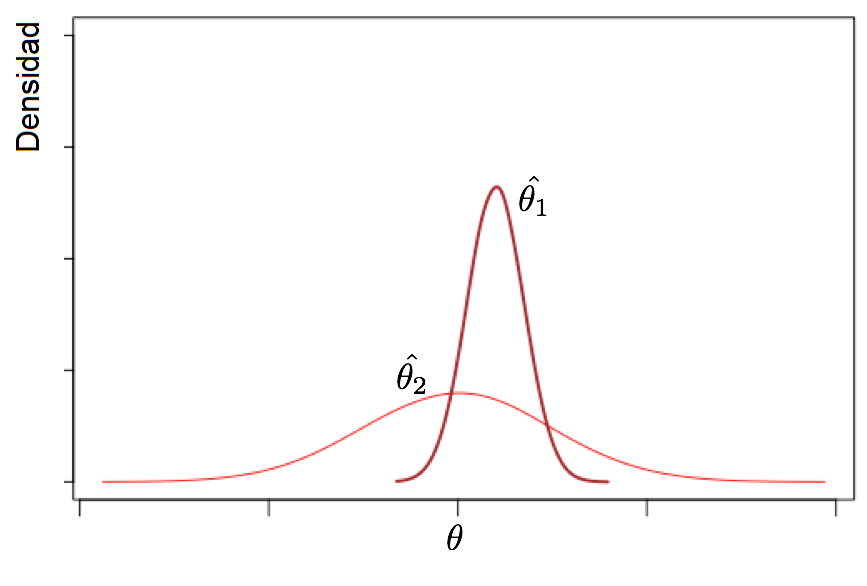
\includegraphics[height=.4\textheight]{slides3/img/biasvariance.png}
  \end{figure}
  \begin{itemize}
    \item En este caso si bien $\widehat{\theta}_2$ es un estimador insesgado para $\theta$ podemos ver del gráfico que su distribución tiene mucha mayor variabilidad que $\widehat{\theta}_1$. Una forma de tomar en cuenta ambas cosas (valor del $\text{sesgo}^2$ + variabilidad de un estimador) es el \textbf{error cuadrático medio}. %El ECM s\'i mide en cierto sentido que un estimador est\'e cerca o lejos del par\'ametro de interés (discutimos un un ejemplo--ver slide 14-- de un estimador sesgado que puede ser mejor que otro insesgado, ya que para algunos valores del parámetro el primero tiene menor ECM).
 % \item Toda una \'area de la estad\'istica moderna estudia maneras
 %   inteligentes de balancear sesgo y varianza para tener un ECM bajo.
  \end{itemize}
\end{frame}

\begin{frame}{\color{rosee}\small Posibles combinaciones de sesgo y varianza de un estimador}
  \begin{figure}
    \centering
    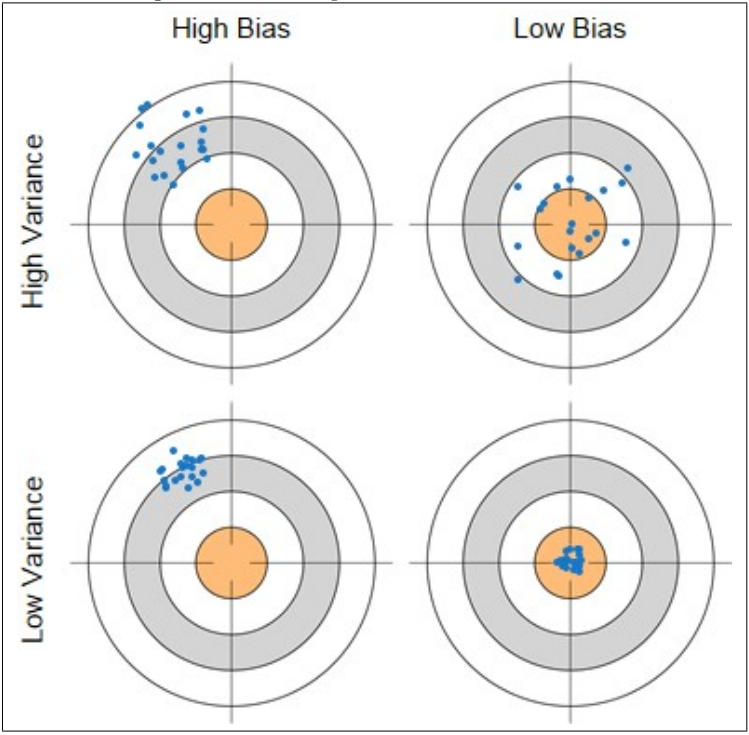
\includegraphics[height=.77\textheight]{slides3/img/bias_var.png}
    \caption{Entre estos cuatro estimadores ¿cómo los rankearíamos?}
  \end{figure}
\end{frame}



\begin{frame}{\color{rosee}Error cuadr\'atico medio} \small \begin{itemize}
       \item  Dado $\widehat{\theta}_n$, un estimador de $\theta$, definimos su
    \textbf{error cuadr\'atico medio (ECM)} como
    \[\text{ECM}(\widehat{\theta}_n,\theta) = E\left[ \left(\widehat{\theta}_n - \theta\right)^{2} \right]\]
  
  \noindent donde $\widehat{\theta}_n-\theta$ es conocido como el \textbf{error de estimaci\'on}.\footnote{También se puede considerar el valor absoluto del error de estimación $ \vert \widehat{\theta}_n - \theta \vert$ y donde $E( \vert \widehat{\theta}_n - \theta \vert)=MAE(\widehat{\theta}_n,\theta)$ se conoce como el \textit{mean absolute error}, a veces se menciona en Métodos Estadísticos y en Econometría.}
  
 \item   \textbf{Idealmente}, buscamose estimadores $\widehat{\theta}_n$ de manera que estas v.a. tengan \textbf{centro de masa} cerca de cero y que su varianzas sean pequeñas.

  

 \item  El ECM es una cantidad que depende (en la mayoría de los casos) de $\theta$ en la población y del tamaño de la muestra $n$.
  \end{itemize}
\end{frame}


\begin{frame}{\color{rosee}Descomposición del Error Cuadr\'atico Medio} \small
  \begin{theorem}[Descomposici\'on del ECM]
    \[ECM(\widehat{\theta}_n,\theta)=E\left[ \left(\widehat{\theta}_n - \theta\right)^{2} \right] =
    \underbrace{\left(E(\widehat{\theta}_n)-\theta\right)^{2}}_{\text{sesgo al cuadrado}} + \underbrace{Var(\widehat{\theta}_n)}_{\text{varianza}}\,.\]
  \end{theorem}
 Calculamos el ECM sumando el $\text{sesgo}^2$ y la var. del estimador, no por definición.
  
  \begin{proof}
    Si llamamos $e = \widehat{\theta} - \theta$. Sabemos que
    \[Var(e) = E\left(e^{2}\right) - \left[E(e)\right]^{2}.\]
    Luego
    \[ ECM(\widehat{\theta}_n,\theta)=E\left(e^{2}\right) = \left[ E(e)\right]^{2} + Var(e).\]
    Adem\'as, como $\theta$ es constante, $E(e) = E(\widehat{\theta}_n) - \theta$ y
    $Var(e) = Var(\widehat{\theta}_n)$.
  \end{proof}
\end{frame}


\begin{frame}{\color{rosee}Comentarios sobre ECM}

  \begin{itemize}
   \item Si $\widehat{\theta}_n$ es insesgado para $\theta$, luego: $\text{ECM}(\widehat{\theta}_n,\theta) = \text{Var}(\widehat{\theta}_n)$.
    \item Un estimador con sesgo y varianza pequeño tiene un ECM pequeño. En otras palabras, la distribución de probabilidad de  $\widehat{\theta}_n$ está \textit{concentrada} en torno de  $\theta$, o lo que es lo mismo, con alta probabilidad el estimador $\widehat{\theta}_n$ toma valores \textit{cerca} del parámetro $\theta$.\medskip
 
    \item Para un valor de $n$ fijo, consideramos dos estimadores de $\theta$ ($\widehat{\theta}_{1}$ y $\widehat{\theta}_{2}$) y comparamos sus ECM. Si se tiene que $\text{ECM}(\widehat{\theta}_{1},\theta) <\text{ECM}(\widehat{\theta}_{2},\theta)$ para todo posible valor de $\theta$, entonces se \textbf{prefiere} $\widehat{\theta}_{1}$ a $\widehat{\theta}_{2}$ como estimador de $\theta$. 
    

     \item Veamos el siguiente ejemplo para determinar qué estimador se prefiere para $\theta$ si el modelo estadístico es $Unif(0,\theta)$.
      
 
      \end{itemize}
      

\end{frame}



\begin{frame}{\color{rosee} ¿Qué estimador de $\theta$ preferimos? Comparación con ECM}
  \small
    Sean $X_i\stackrel{iid}{\sim} Unif(0,\theta)$, dos estimadores consistentes de $\theta$ son
    \[\widehat{\theta}_{n,1}=\max\{X_{1},\dots, X_{n}\} \quad \text{ y } \quad \widehat{\theta}_{n,2}=2\overline{X}_n\]
    
    Recuerde que 
    \[ \scalebox{0.95}{$E(\widehat{\theta}_{n,1})=\frac{n}{n+1}\theta, E(\overline{X}_n)=\frac{\theta}{2}, Var(\widehat{\theta}_{n,1})=\frac{n\theta^2}{(n+1)^2(n+2)}, Var(\overline{X}_n)=\frac{\theta^2}{12n}$}\]
    
    Para decidir qué estimador de $\theta$ prefiere, compare los ECM de:
    \begin{enumerate}[label=(\alph*)]
        \item  $\widehat{\theta}_{n,1}$ y $\widehat{\theta}_{n,2}$.
        \item $\widehat{\theta}_{n,1}$ y $\frac{n+1}{n}\widehat{\theta}_{n,1}$
    \end{enumerate}

\color{gray}
En (a) se prefiere $\widehat{\theta}_{n,1}$ si $n \geq 3$.  En (b) se prefiere $\frac{n+1}{n}\widehat{\theta}_{n,1}$ si $n \geq 2$.
\begin{align*}
    ECM(\widehat{\theta}_{n,1})=&\frac{\theta^2}{(n+1)^2}+\frac{n\theta^2}{(n+1)^2(n+2)}=\frac{2\theta^2}{(n+1)(n+2)}\\ ECM(\widehat{\theta}_{n,2})=&\frac{\theta^2}{3n} \quad  \text{ y } \quad ECM\left( \frac{n+1}{n}\widehat{\theta}_{n,1}\right)=\frac{\theta^2}{n(n+2)}
\end{align*}

%RECORDAR QUE $\frac{n+2}{n+1}\widehat{\theta}_{n,1}$ tiene $ECM=\frac{\theta^2}{(n+1)^2}$ que es el menor ECM de los estimadores que son multiplos del max de las $X_i$

  
\end{frame}

%%%%% ECM no es un criterio que sirva para comparar siempre estimadores

\begin{frame}{\color{rosee} \small Ejemplo X: Comparar estimadores usando el ECM no siempre es concluyente} \small 
  
Dada una muestra aleatoria $X_{1},\dots, X_{n} \sim \text{Ber}(p)$, coinsideremos los siguientes tres estimadores de $p=E(X)$:
    \begin{itemize}
    \item La media muestral: \[\widehat{p}_{1}=  \overline{X}_{n}\,.\]
    \item La media muestral agregando $2$ fracasos y $2$ \'exitos
      ``artificiales'' a la muestra:
      \[\widehat{p}_{2} = \frac{ \sum_{i=1}^{n}X_{i} + 2}{n+4}\,.\]
    \item La media muestral de s\'olo dos observaciones:
      \[\widehat{p}_{3} = \frac{X_{1}+X_{2}}{2}\,.\]
    \end{itemize}
  Sabemos que $\widehat{p}_{1}$ es consistente para $p$ por LGN para $X_i\stackrel{iid}{\sim}$ y por propiedades de convergencia en probabilidad $\widehat{p}_{2}$ es consistente para $p$. Por otro lado, $\widehat{p}_{3}$ no es consistente para $p$. Descartamos $\widehat{p}_{3}$, pero ¿c\'omo determinamos si preferimos estimar a $p$ usando $\widehat{p}_{1}$ o $\widehat{p}_{2}$? \textbf{Calculemos el ECM de cada estimador.}
\end{frame}


\begin{frame}{\color{rosee}Ejemplo X: \color{orang} ECM$(\widehat{p}_{1},p)$ \color{rosee}vs. \color{dodgerblue} ECM$(\widehat{p}_{2},p)$}
      Como $\left(\widehat{p}_{1}\right) =  p \text{ y } Var(\widehat{p}_{1})=\frac{p(1-p)}{n}$, entonces el ECM de $\widehat{p}_{1}$ es
    \[\color{orang}ECM\left(\widehat{p}_{1},p \right)=\frac{p(1-p)}{n}.\]
Para calcular el ECM de $\widehat{p}_{2}$, sabemos que
      \[E\left(\widehat{p}_{2}\right) =  \frac{np+2}{n+4}\text{ y } Var(\widehat{p}_{2})=\frac{np(1-p)}{(n+4)^2}\]
      
      Entonces el ECM de $\widehat{p}_{2}$ es
      \[\color{dodgerblue}\text{ECM}(\widehat{p}_2,p) 
      = E\left( (\widehat{p}_{2} - p)^{2} \right)=
        \left(\frac{2(1 -2p)}{n+4}\right)^2
        + \frac{np(1-p)}{(n+4)^{2}}.\]

      \textbf{     ¿Qué estimador preferimos? }

 Si uno de los dos ECM fue menor para todos los valores
    de $n\in \NN$ (o al menos si $n\to +\infty$) y de $p\in (0,1)$, ese ser\'ia el estimador preferido.
    
Graficando los ECM veremos que no podemos elegir, bajo este criterio, un estimador que prefiramos usar para estimar a $p$.
%Ayuda: Recuerden que la suma de $n$ v.a. independientes Bernoulli da como resultado una variable aleatoria Binomial; por lo tanto $T\sim Bin(n,p)$ y por esto último $E(T)=np$ y $Var(T)=np(1-p)$.
\end{frame}


\begin{frame}{\color{rosee}Ejemplo X: \color{orang} ECM$(\widehat{p}_{1},p)$ \color{rosee}vs. \color{dodgerblue} ECM$(\widehat{p}_{2},p)$}\small
\begin{columns}
  \begin{column}{7cm}
      \begin{figure}
    \centering
    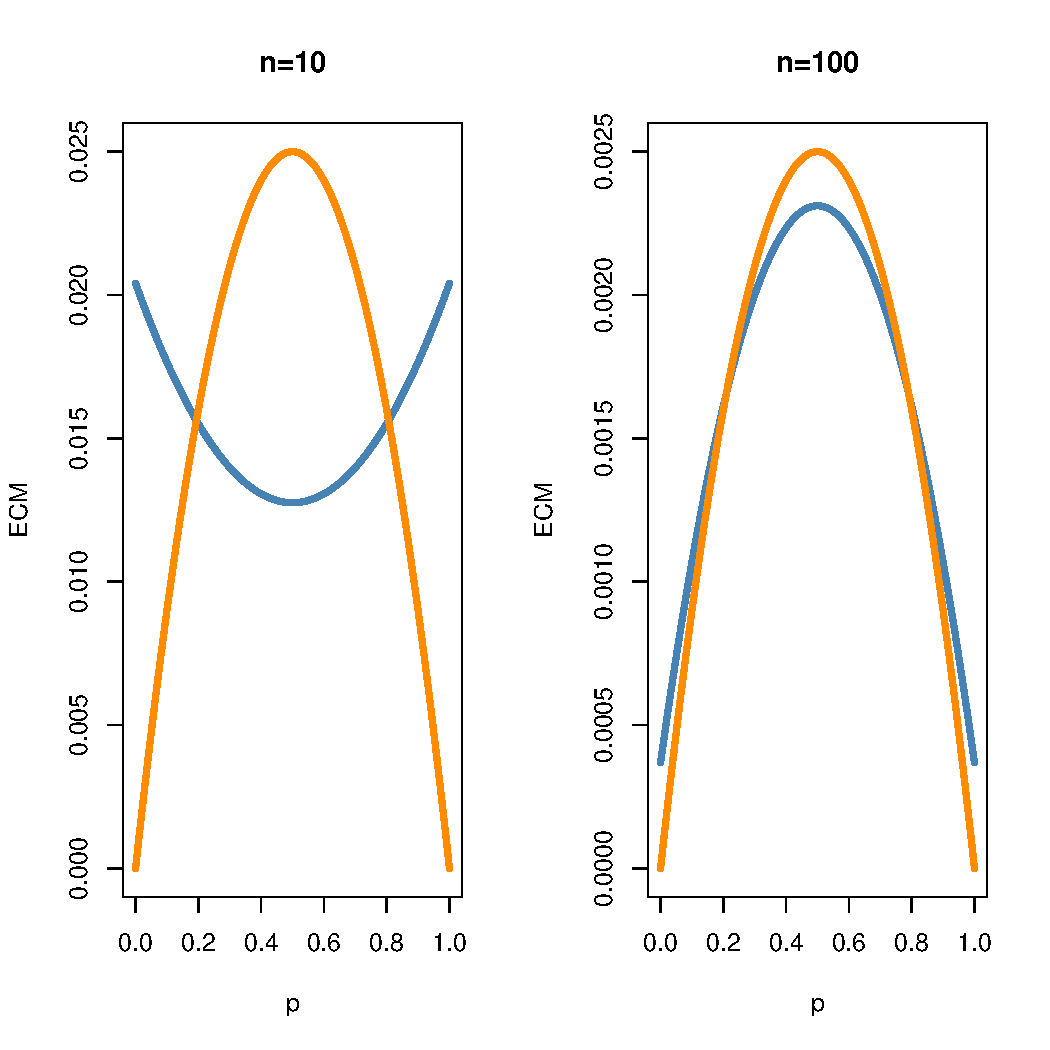
\includegraphics[height=.6\textheight]{slides3/img/ECM-bernoulli.pdf}
    \caption{\small\color{orang}$ECM(\widehat{p}_{1},p)$ (naranja) \color{black} y \color{dodgerblue}
      $ECM(\widehat{p}_{2},p)$ (azul)\color{black}.}
  \end{figure}
  \end{column}
  \begin{column}{5cm}
   { \small Podemos concluir que el estimador \color{dodgerblue}$\widehat{p}_2$ tendrá menor ECM para valores de $p$ cercanos a $\frac{1}{2}$ \color{black} para cualquier tamaño de muestra $n$ y por lo tanto no podemos descartarlo como potencial estimador de $p$. Por otro lado, \color{orang} para valores alejados de $p=\frac{1}{2}$ el estimador $\overline{X}_n$ tiene menor ECM\color{black}.}
  \end{column}
\end{columns}
\end{frame}

\begin{frame}{\color{rosee}Error cuadr\'atico medio y optimalidad de un estimador}
 
    \begin{itemize}
    \item No siempre existe un estimador ``mejor'' que todos los demás estimadores para el parámetro $\theta$. Es decir, no siempre existe un estimador que tenga un ECM menor que el de cualquier otro estimador de $\theta$, para cualquier valor de $\theta$. \medskip
    
    \item  Sin embargo, si limitamos los estimadores que consideramos, por ejemplo para el modelo estadístico $X_i\stackrel{iid}{\sim} U(0,\theta)$ si consideramos los estimadores $\widehat{\theta}_{k}=k\max\{X_1, \cdots ,X_n \}$ se cumple que \[\widehat{\theta}_{\frac{n+2}{n+1}}=\frac{n+2}{n+1}\max\{X_1, \cdots ,X_n \}\] tiene ECM$\left(\widehat{\theta}_{\frac{n+2}{n+1}},\theta\right)=\frac{\theta^2}{(n+1)^2}$ que es el menor ECM para esa familia de estimadores de $\theta$.
 
    \end{itemize}
  
\end{frame}


\begin{frame}{\color{rosee}Estimadores insesgados con mayor eficiencia}
        
    \begin{itemize}
  \item  Dados dos estimadores \underline{insesgados} $\widehat{\theta}_n$ y
    $\widetilde{\theta}_n$ de $\theta$, decimos que $\widehat{\theta}_n$ es
    m\'as \textbf{eficiente} que $\widetilde{\theta}_n$ si
    \[Var(\widehat{\theta}_n) \leq Var(\widetilde{\theta}_n).\]
      \item Entre dos estimadores insesgados, será mejor aquel que tenga la menor varianza (y por lo tanto el menor ECM).
      \item Definimos la \textbf{eficiencia relativa} entre dos \textbf{estimadores insesgados} $\widehat{\theta}_n$ y $\widetilde{\theta}_n$ como
      \[ER(\widehat{\theta}_n,\widetilde{\theta}_n)=\frac{Var(\widehat{\theta}_n)}{Var(\widetilde{\theta}_n)}\]
      \item Preferimos $\widehat{\theta}_n$ (a $\widetilde{\theta}_n$) para estimar a $\theta$ si $ER(\widehat{\theta}_n,\widetilde{\theta}_n)<1$.
  \end{itemize}
  
  %  Si $\widehat{\theta}_n$ es m\'as eficiente que  $\widetilde{\theta}_n$, entonces $\widehat{\theta}_n$ usa mejor la  informaci\'on en la muestra que $\widetilde{\theta}_n$. Notar también que si $\widehat{\theta}_n$ es más eficiente que $\widetilde{\theta}_n$, entonces el ECM del primer estimador es menor que el del segundo estimador.
  
  
  
\end{frame}



\begin{frame}{\color{rosee}Eficiencia relativa - ejemplo}\small
 
    {\small$2{\overline{X}_{n}}$} y
    {\small$\frac{n+1}{n} \widehat{\theta}_{n,1}$} son insesgados para $\theta$ cuando {\small $X_1,\dots,X_n\stackrel{iid}{\sim} Unif(0,\theta)$}. Recordemos que:\medskip
    \begin{itemize}[leftmargin=*]
        \item $ECM\left(\frac{n+1}{n} \widehat{\theta}_{n,1},\theta\right)=Var\left(\frac{n+1}{n}
      \widehat{\theta}_{n}\right)=\left(\frac{n+1}{n}
    \right)^{2}Var(\widehat{\theta}_{n}) = \frac{\theta^{2}}{n(n+2)}$
    \item $ECM\left(2{\overline{X}_{n}},\theta\right)=Var\left(2{\overline{X}_{n}}\right)=4 Var(\overline{X}_{n}) =
    \frac{4}{n} Var(X_{1})=\frac{4}{n} \frac{\theta^{2}}{12} =
    \frac{\theta^2}{3n}$
    \end{itemize}
    Luego para todo $n>1$ y para todo $\theta$ se cumple que:
    \[Var(\widetilde{\theta}_n) = \frac{\theta^{2}}{n(n+2)} \leq \frac{\theta^{2}}{3n} = Var(2{\overline{X}_{n}})\,.\]
  

    Entonces concluimos que $\frac{n+1}{n} \widehat{\theta}_{n}$
    es m\'as eficiente que $2{\overline{X}_{n}}$ y lo preferimos para estimar a $\theta$. \textbf{Por otro lado}, notemos que si $n\to +\infty$, la varianza de
    $\widetilde{\theta}_{n}$ es mucho m\'as chica que la de
    $2{\overline{X}_{n}}$. De hecho
    \[\frac{Var(\widetilde{\theta}_{n})}{Var(2{\overline{X}_{n}})} \ton 0.\]
 
\end{frame}

\begin{frame}{\color{rosee}Estimadores insesgados de m\'inima varianza} \small

\begin{itemize}
    \item Consideremos todos los estimadores insesgados de $\theta$. ¿Podemos determinar si hay un estimador ``mejor'' para estimar a $\theta$? No siempre, pero si existe se conoce como IMV. 
  \item \textbf{Definición:} Entre todos los estimadores de $\theta$ que son insesgados, el que
    tiene m\'inima varianza se denomina \textbf{estimador insesgado de
      m\'inima varianza (IMV)}. El estimador IMV es el que minimiza el ECM entre los estimadores insesgados de $\theta$.
\item  No vamos a ver en el curso como obtener estimadores IMV.
%  \begin{alertblock}{Idea}
   % El IMV es, de todos los insesgados, el que tiene una distribuci\'on    muestral con menor dispersi\'on alrededor de $\theta$. Entonces, como sabemos que el ECM es la suma de la varianza del estimador y de su sesgo al cuadrado, el estimador IMV es el que minimiza el ECM   entre los insesgados.
%  \end{alertblock}
  \item \textbf{Ejemplo 1:} Para el modelo $X_i\stackrel{iid}{\sim}N(\mu,\sigma^2)$, vale que $\overline{X}_n$ es IMV para $\mu$.
  \item \textbf{Ejemplo 2:} Para el modelo $X_i\stackrel{iid}{\sim}U(0,\theta)$, vale que $\frac{n+1}{n}\max\{X_1,\cdots, X_n\}$ es IMV para $\theta$ (antes solo hab\'iamos mostrado que era m\'as
    eficiente que $2\overline{X}_{n}$).
\end{itemize}
Más adelante estudiaremos una familia de estimadores (los de máx. verosimilitud) que tienen mínima
varianza \textbf{asintótica}, que es el tipo de optimalidad relevante
para construir intervalos de confianza y tests de hipótesis.

\end{frame}



\begin{frame}{\color{rosee} Estimador BLUE: definición y ejercicio}

\begin{itemize}
    \item Se llama estimador lineal a un estimador que surge de sumar v.a. y multiplicar por constantes. Por ejemplo, si se tiene $X_i\stackrel{iid}{\sim}$ e $Y_i\stackrel{iid}{\sim}$ un estimador lineal de $E(X)$ es $\alpha \overline{X}_n + \beta \overline{Y}_n$.
    
\item Decimos que un \textbf{estimador es BLUE} (best linear unbiased estimator) si es \textbf{lineal, insesgado y tiene la menor varianza} entre los estimadores lineales y insesgados.
\end{itemize}
Se busca estimar $p$, la proporción de personas que van a votar a Azucena Novoy. Se tienen, para estimar a $p$, dos muestras aleatorias $X_1,\dots , X_n$ e $Y_1, \dots , Y_n$. Se considera el siguiente estimador lineal de $p$:
$$\widehat{p} = \alpha \overline{X}_n + \beta \overline{Y}_n.$$

\begin{enumerate}
    \item Encuentre los valores de $\alpha$ y $\beta$ para los que $\widehat{p}$ es un estimador insesgado y consistente de $p$. \color{gray} $\alpha+\beta=1$ \color{black}\medskip
    \item ¿Para qué valores de $\alpha$ y $\beta$ se minimiza la varianza de $\widehat{p}$, sujeto a que $\widehat{p}$ sea un estimador insesgado de $p$? \color{gray} $\alpha=\beta=\frac{1}{2}$ \color{black} 
\end{enumerate}
\end{frame}


\begin{frame}{\color{rosee}Error est\'andar de un estimador}\small
%  Adem\'as de reportar la estimaci\'on (puntual) debemos indicar su precisi\'on.
  \begin{itemize}
      \item  El \textbf{error est\'andar} de un estimador $\widehat{\theta}_n$
    es el desv\'io est\'andar de $\widehat{\theta}_n$. Es decir, $\text{se}(\widehat{\theta}_n)=
    \sqrt{Var(\widehat{\theta}_n)}$.
  
 \item Un estimador de un parámetro $\theta$ es una variable aleatoria que tiene cierta variabilidad. En general, esa variabilidad depende de $\theta$ o de otros parámetros desconocidos.
 
 \item Es por eso que buscaremos estimadores de $
    \sqrt{Var(\widehat{\theta}_n)}$
   % \item Si repetimos el experimento, cambia la muestra y posiblemente cambie  el valor estimado del parámetro. El error est\'andar cuantifica la variabilidad del estimador del parámetro de interés.\medskip
   % \item El error estándard es una cantidad fija que en algunos casos podremos calcular exactamente y en otros,     la mayor\'ia, tendremos que estimar.\medskip
      \item Llamamos $\widehat{\text{SE}}(\widehat{\theta}_n)$ a un \textbf{estimador} de $\sqrt{Var(\widehat{\theta}_n)}$.
      
      \item Llamamos  $\widehat{\text{se}}(\widehat{\theta}_n)$ a una \textbf{estimación puntua}l de $\sqrt{Var(\widehat{\theta}_n)}$ usando $\widehat{\text{SE}}(\widehat{\theta}_n)$ a partir de los datos disponibles. 
          \end{itemize}
  
\end{frame}

\begin{frame}{\color{rosee}Error est\'andar de $\overline{X}_n$} \small
\begin{itemize}[leftmargin=*]
    \item  Para un modelo estadístico cualquiera, consideramos $\overline{X}_n$ un estimador de $E(X)$.
  \item  El error est\'andar de $\overline{X}_{n}$ es:
    \[\text{se}(\overline{X}_{n}) = \sqrt{Var\left(\overline{X}_{n}\right)}= \frac{\sqrt{Var(X)}}{\sqrt{n}},\]
    que depende de $Var(X)$. Dos estimadores consistente de $\sqrt{Var(X)}$ son
    \begin{itemize}
        \item $\widehat{\sigma}_n= \sqrt{\frac{1}{n} \sum_{i=1}^{n}X_{i}^{2}
      - \left(\overline{X}_{n}\right)^{2}}$
      \item $S_n= \widehat{\sigma}_n \sqrt{\frac{n}{n-1}}$
    \end{itemize}
    
    \item Dos posibles maneras de estimar el error est\'andar de $\overline{X}_{n}$ son:
    \begin{itemize}
        \item  $\widehat{\text{SE}}(\overline{X}_{n}) = \frac{\widehat{\sigma}_n}{\sqrt{n}}$
        \item  $\widehat{\text{SE}}(\overline{X}_{n}) = \frac{S_n}{\sqrt{n}}$
    \end{itemize}
  %  $\widehat{\text{SE}}(\overline{X}_{n}) = \frac{\widehat{\sigma}_n}{\sqrt{n}}$. Para unos datos en concreto, tendremos una estimación puntual de la raíz de la varianza en la población y con ello una estimación puntual del error estándar asociado a $\overline{X}_{n}$.
  
  \end{itemize}

\end{frame}

\begin{frame}{\color{rosee}Error est\'andar de $\overline{X}_n$ - ejercicio 1}\small
  
    En el proceso de ensamblaje de celulares en una f\'abrica se cometen
    errores. El n\'umero de rayaduras en la pantalla de un celular
    elegido al azar de la l\'inea de montaje es una variable aleatoria
    $X$ con distribuci\'on Poisson de par\'ametro $\lambda$. Se toma una
    muestra aleatoria de $150$ celulares y se registran los siguientes
    resultados:
% , donde la primer fila indica el n\'umero de rayaduras y
%     la segunda la frecuencia observada. Por ejemplo, hubo 42 celulares
%     en la muestra con 2 rayaduras en la pantalla.
    \begin{table}
      \centering
      \begin{tabular}{|r|rrrrrrrr|}
        \hline
        \mbox{n\'umero de rayaduras}&0&1&2&3&4&5&6&7\\
        \mbox{ocurrencias en la muestra}&18&37&42&30&13&7&2&1\\
        \hline
      \end{tabular}
    \end{table}
    \begin{itemize}
    \item Proponga un estimador consistente e insesgado para
      $\lambda$. Calcule el valor estimado obtenido para esta muestra.
    \item Proponga un estimador consistente para la varianza
      de $X$. Proponga un estimador para el error est\'andar del
      estimador propuesto en el item anterior. ¿C\'ual es la estimación puntual del error
      est\'andar para los datos de esta muestra?
    \end{itemize}
  
\end{frame}

\begin{frame}{\color{rosee}Error est\'andar de $\overline{X}_n$ - ejercicio 2}\small
  
Considere la variable aleatoria $X$ que en la población argentina toma el valor $1$ cuando una familia en los últimos 3 meses vivió de ayudas sociales o subsidios del gobierno, la iglesia, etc; y $0$ en otro caso. La siguiente tabla tiene los datos de la EPH (1T--2021) de una muestra de familias argentinas:% (ver columna V5):
    \begin{table}
      \centering
      \begin{tabular}{|l|cc|}
        \hline
        \mbox{Valores de X }&0&1\\
        \hline
        \mbox{ocurrencias en la muestra}&12897 & 2521\\
        \hline
      \end{tabular}
    \end{table}
    \begin{itemize}
    \item Proponga un estimador consistente e insesgado para
      $E(X)$. Calcule el valor estimado obtenido para esta muestra.
    \item Proponga un estimador consistente para la varianza
      de $X$. Proponga un estimador para el error est\'andar del
      estimador propuesto en el item anterior. ¿C\'ual es la estimación puntual del error
      est\'andar para los datos de esta muestra?
    \end{itemize}
  
\end{frame}



\end{document} 
